\documentclass[conference]{IEEEtran}
\IEEEoverridecommandlockouts
% The preceding line is only needed to identify funding in the first footnote. If that is unneeded, please comment it out.
\usepackage{cite}
\usepackage{amsmath,amssymb,amsfonts}
\usepackage{algorithmic}
\usepackage{graphicx}
\usepackage{textcomp}
\usepackage{xcolor}
\usepackage{url}
\usepackage{array}
% \def\BibTeX{{\rm B\kern-.05em{\sc i\kern-.025em b}\kern-.08em
%     T\kern-.1667em\lower.7ex\hbox{E}\kern-.125emX}}
\begin{document

\title{SURVEY OF LSM TREES AND INDEXING TECHNIQUES IN KEY-VALUE STORES\\
{\footnotesize \textsuperscript{}}
% \thanks{979-8-3315-5418-7/25/\$31.00 ©2025 IEEE}
}


\author{
\IEEEauthorblockN{1\textsuperscript{st} Chaitanya Paraskar}
\IEEEauthorblockA{\textit{Department of Computer Engineering} \\
\textit{Pune Institute of Computer Technology}\\
Pune, India \\
cvparaskar2004@gmail.com}
\and
\IEEEauthorblockN{2\textsuperscript{nd} Shreyash Dhas}
\IEEEauthorblockA{\textit{Department of Computer Engineering} \\
\textit{Pune Institute of Computer Technology}\\
Pune, India \\
shreyashrdhas@gmail.com}
\and
\IEEEauthorblockN{3\textsuperscript{rd} Shreyash Gajbhiye}
\IEEEauthorblockA{\textit{Department of Computer Engineering} \\
\textit{Pune Institute of Computer Technology}\\
Pune, India \\
shreyashgajbhiye90@gmail.com}
\and
\IEEEauthorblockN{4\textsuperscript{th} Shreyas Gopnarayan}
\IEEEauthorblockA{\textit{Department of Computer Engineering} \\
\textit{Pune Institute of Computer Technology}\\
Pune, India \\
gopnarayanshreyas2004@gmail.com}
\and
\IEEEauthorblockN{5\textsuperscript{th} Prof. Madhuri Mane}
\IEEEauthorblockA{\textit{Department of Computer Engineering} \\
\textit{Pune Institute of Computer Technology}\\
Pune, India \\
mvmane@pict.edu}
}

\maketitle
\begin{abstract}
Log-Structured Merge (LSM) trees form the backbone of many modern key-value stores, offering a write-optimized storage model well-suited for applications with high update rates. As these systems evolve to meet diverse performance requirements, the design of indexing mechanisms—particularly those affecting read efficiency—has emerged as a critical area of study. This survey provides a structured overview of LSM-tree-based storage architectures, with a focus on optimization strategies for primary and secondary key access.

We begin by outlining the core components of LSM trees, including memtables, write-ahead logs, SSTables, Bloom filters, and sparse indexes. The discussion then extends to a range of key-value stores and database systems—such as LevelDB, RocksDB, Cassandra, HBase, and AsterixDB—each illustrating distinct trade-offs in compaction policy, memory hierarchy, and indexing structure. In parallel, the paper reviews emerging adaptations involving persistent memory, disaggregated memory systems, hybrid storage layouts, and key-value separation.

Through comparative analysis of these systems and techniques, the paper reviews a wide spectrum of architectural approaches employed in current LSM-based engines. While not prescriptive in nature, the survey offers a comprehensive reference point for understanding architectural trends and indexing optimizations in write-intensive storage environments.
\end{abstract}

\begin{IEEEkeywords}
Log-Structured-Merge Trees, Key-Value Stores, Indexing, Primary Indexing, Secondary Indexing
\end{IEEEkeywords}

\begin{figure*}[htbp]  
    \centering
    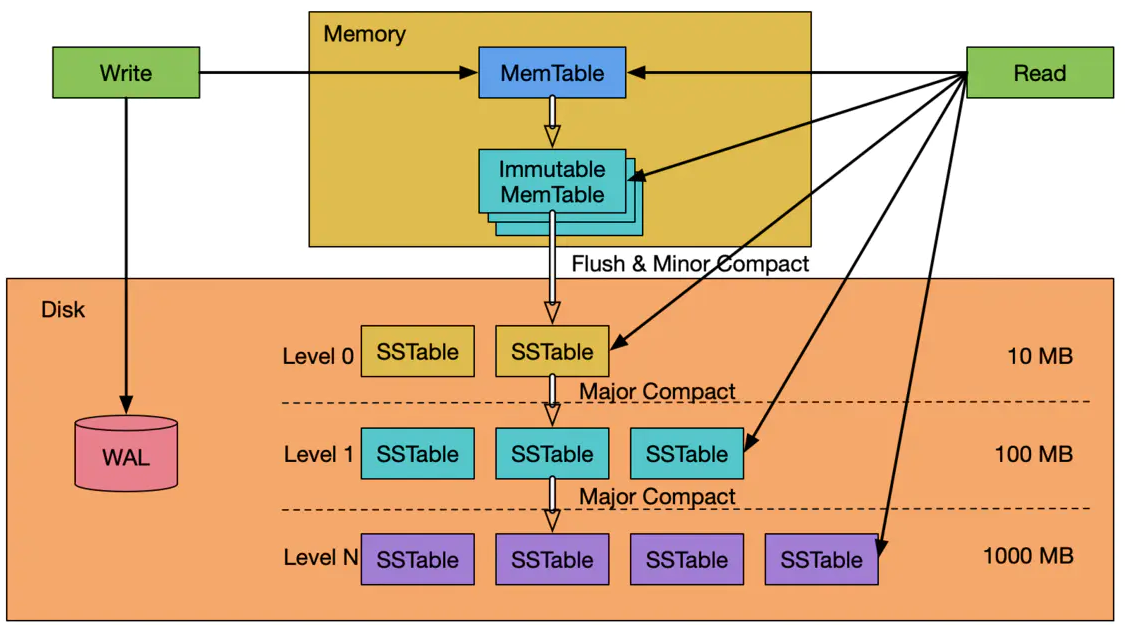
\includegraphics[width=\textwidth, height=12cm]{LSM- Architecture.png} 
    \caption{LSM Tree Architecture Diagram} 
    \label{fig:fullpage_image}
\end{figure*}

% \section{Introduction}
% \label{sec:introduction}
% Log-Structured Merge (LSM) Tree-based key-value stores have become essential to modern data systems. They support applications that need high ingest rates, real-time analytics, and predictable scalability. Their design focuses on grouping writes in memory and writing large sequential segments to disk. This approach works especially well in environments with constant data creation, like IoT systems, logging setups, and large online services. As a result, LSM-based engines like RocksDB, LevelDB, Cassandra, and HBase now form the backbone of many production systems in both industry and academia.

% However, LSM trees come with it's own challenges. The multi-level arrangement of SSTables can lead to more read amplification, increased query latency, and extra operational work during compaction. These issues are more serious for workloads that need efficient non-primary-key access or quick point queries. Recent research has focused on developing improvements, from better compaction methods to hybrid memory setups and new indexing structures, to find a better balance between write-optimized designs and read performance.

% This survey looks closely at these developments. We examine traditional leveled and tiered compaction strategies, compare popular LSM-based systems, and explore new solutions like persistent-memory-enhanced indexing (Perseid), hybrid storage engines (SpanDB), and multi-index architectures (AsterixDB). By reviewing the changes in both primary and secondary indexing in LSM stores, this paper aims to highlight current limitations, point out promising advancements, and lay the groundwork for the next generation of key-value storage systems.

\section{Introduction}
Key-value stores have become a foundational component in modern data infrastructure, underpinning a broad range of latency-sensitive applications—from cloud-native services and real-time analytics to embedded systems and distributed platforms. Among the various storage architectures, Log-Structured Merge (LSM) trees have emerged as the preferred design for write-intensive workloads due to their ability to transform random writes into sequential disk operations and scale efficiently with growing data volumes [1][3].

Despite their widespread adoption, LSM-tree-based systems are inherently read-unfriendly. The compaction hierarchy, while effective for write throughput and space utilization, leads to significant read amplification, latency variability, and complex maintenance overheads [3][13]. These challenges are especially pronounced in workloads that require secondary-key lookups or range queries, where multi-level SSTable traversal and obsolete entry filtering become performance bottlenecks [2][14].

Recent research and system-level innovations have sought to address these limitations through various architectural and indexing enhancements. Key-value engines like RocksDB, Cassandra, HBase, and LevelDB serve as practical case studies for core LSM design trade-offs [5][7][8][28], while newer systems such as Perseid [14], NVKVS [7], and SpanDB [12] explore hybrid memory models and disaggregated architectures to improve both indexing efficiency and I/O behavior. Meanwhile, AsterixDB exemplifies the integration of multi-index structures—B+ trees, inverted indexes, and R-trees—within a unified LSM framework to support analytical workloads at scale [16][17].

This survey presents a comprehensive review of primary and secondary indexing strategies employed in LSM-based key-value stores, examining the evolution of index organization across memory and disk layers. It explores the role of memtables, WALs, bloom filters, sparse indexes, and recent techniques such as persistent memory-based indexing and NV-cache acceleration. The goal is to provide a survey of current design limitations and the emerging directions aimed at improving lookup performance without compromising write efficiency. By synthesizing these advances, the paper offers insights into the architectural decisions that define the next generation of high-performance, LSM-centric data storage systems.

\section{LSM-Tree Architecture}
Log-Structured-Merge (LSM) trees are the basis of many modern write-optimized key-value stores. They separate in-memory buffering from on-disk storage. This design turns random I/O into sequential operations and allows for quick lookups using additional indexing structures. The key parts that make this architecture work are memtables, write-ahead logs, SSTables, bloom filters, and sparse indexes.[1]
\subsection{\textbf{Memtable}}
The Memtable is an in-memory structure that temporarily collects incoming writes in a sorted format. By buffering inserts, updates, and deletes in DRAM, it reduces the cost of random disk writes and changes them into sequential flushes. When the Memtable fills up, its contents are saved as a new SSTable on the disk. This temporary buffer allows quick access to recently written keys and supports high write speeds. Implementations usually use skip lists or balanced trees to keep the sorted order while allowing efficient lookups and inserts. Overall, the Memtable handles high write rates and supports scalable LSM-tree performance.[1]
\subsection{\textbf{Write-Ahead Log (WAL)}}
The Write-Ahead Log records every update before it gets applied to the Memtable, ensuring durability. As an append-only structure, the WAL reduces disk seek time and offers a reliable recovery method if there are system crashes. When the system restarts, unpersisted Memtable updates can be rebuilt by replaying the WAL. This sequential logging method maintains throughput while ensuring strong crash consistency. Techniques like batching and optimized fsync handling further cut down overhead. The WAL thus maintains high write performance while ensuring strong fault tolerance in LSM-based systems.[1]
\subsection{\textbf{SSTables}}
Sorted String Tables (SSTables) are unchangeable, disk-based components that keep sorted key-value pairs flushed from the Memtable. Their append-only creation allows for high-speed sequential writes, while their unchangeable nature makes concurrency control easier. SSTables enable efficient range scans, binary searches, and metadata like Bloom filters and sparse indexes for quicker queries. They are usually organized in multiple levels and periodically merged through compaction to manage lookup overhead and reclaim old entries. SSTables provide durable and read-efficient storage while maintaining the write-optimized structure of the LSM design.[1]
\subsection{\textbf{Bloom Filters}}
Bloom filters are small, probabilistic structures linked to SSTables to speed up key lookups. Before accessing the disk, the Bloom filter is checked to see if a key might be in the SSTable. A negative result guarantees that the key is not present, allowing the system to avoid disk I/O entirely. While false positives can happen, Bloom filters greatly reduce read amplification, especially in multi-level LSM structures. By decreasing unnecessary disk probes, they lower latency and improve overall query throughput in large key-value systems.[1]
\subsection{\textbf{Sparse Indexes}}
The use of sparse indexes is possible because sparse indexes allow binary searches and provide a mapping of all blocks in an SSTable within memory rather than needing a mapping of every key in each block. A block of data also includes the first key in the block therefore allowing a sparse index to remain compact while still allowing an efficient way to look up records on disk. When you execute a query on an SSTable, the use of a sparse index allows you to limit your search to only one block of data on the disk, making it easier for a sequential scan to find the corresponding keys quickly. As SSTables become larger in size, sparse indexes help reduce the number of reads from the disk thus decreasing reading latency if used with Bloom filters. It is safe to assume that without using a sparse index, you would not obtain an efficient read using the write-optimized architecture of the LSM.[1]

\section{Survey: LSM-Tree Based Databases}
\vspace{-15pt}
\subsection{\textbf{LevelDB}}
LevelDB [28], developed by Google in 2011, is an embedded key-value storage engine based on the Log-Structured Merge-Tree (LSM-Tree) architecture. It buffers write operations in an in-memory structure called a memtable, which is periodically flushed to disk as immutable, sorted files known as Sorted String Tables (SSTables). LevelDB employs a leveled compaction strategy and the use of partitioned leveled compaction (PLC). It supports basic operations such as insertions, retrievals, and scans, but lacks native support for secondary indexing.
\subsection{\textbf{RocksDB}} 
RocksDB [22][29] by Facebook is an advanced evolution of LevelDB, designed to address high-performance storage requirements. Retaining the foundational LSM-tree architecture RocksDB introduces a range of enhancements aimed at improving both write efficiency and overall system performance. This includes implementation of tiered compaction at level 0, alongside the dynamic adjustment of level sizes relative to the final level, which together serve to reduce both write and space amplification. RocksDB adopted a leaky bucket mechanism [18] to optimize the CPU and disk resources consumption during merge operations.
\subsection{\textbf{Apache HBase}}
HBase [27] is a distributed wide-column databse based on Hadoop Ecosystem and modeled after Google's Bigtable. Data is dynamically partitioned and replicated across multiple regions. Each region has a LSM-tree based storage consisting of a memstore and HFile based SSTables in Hadoop File System (HDFS). HBase supports two data compaction strategies :- Exploring Compaction Policy and Date-Tiered Compaction Policy. The Exploring Compaction Policy includes scanning of all data records and selecting the data records for campaction that minimize write amplification. The Date-Tiered policy is optimized for time-series data. It organizes data based on it's temporal range, resulting in better performance of time based range queries.
\subsection{\textbf{Apache Cassandra}}
Cassandra [26] is a distributed, open-source data management system developed by the Apache Software Foundation. Cassandra is designed to create a scalable and fault-tolerant architecture combining elements from Amazon DynamoDB[19] and Google BigTable[18]. In contrast to systems like HBase, Cassandra eliminates the risk of a single point of failure by employing a fully decentralized design. Data is partitioned and stored using LSM-Trees and supports tiered, leveled, and date-tiered merge policy. Cassandra supports secondary indexes, improving query capabilities on structured data and semi-structured data.
\subsection{\textbf{Apache AsterixDB}}
Apache AsterixDB [16][17] is a Big Data Management System based on an advanced LSM-Tree based storage engine for semi-structured data. The data is partitioned based on hashed primary keys, where each partition is partitioned across multiple nodes. Each node uses an LSM storage layer with a primary index and multiple local secondary indexes. AsterixDB provides a transactional model that ensures consistency across all indexes of a partition. It has an LSM-based B+Tree for normal queries, inverted indexes to support full text and similarity queries, and LSM-based RTree for spatial queries. AsterixDB supports correlated compaction, where all indexes of a dataset are merged together, improving performance for multi-index workloads.

\section{Survey: LSM-Tree based Key-Value Stores}
\vspace{-15pt}
\subsection{\textbf{WiscKey}}
WiscKey [5] is an LSM-tree–based key–value store that separately stores keys and values to mitigate I/O amplification. Keys and value pointers are organized within a sorted LSM-tree, and the actual values are appended to a separate log structure on SSDs. WiscKey decouples large values from the LSM-tree, reducing the size of LSM tree which results in in reduced frequency and cost of compaction. This results in lower write amplification extending the life of SSDs. This design decision contributes to improved write throughput as well as reduced tail latency during i/o operations.
\subsection{\textbf{SpanDB}}
SpanDB [12] is a LSM-tree–based key–value store built on top of RocksDB and tailored for hybrid storage environments. Its partitions the LSM-tree across two storage tiers, placing the write-ahead log and the upper performance-critical levels of the tree on high-speed NVMe SSDs, while storing the lower levels that contain the majority of the data on high-capacity SATA SSDs. This tiered placement strategy preserves RocksDB’s conventional architecture, including sorted memtables in DRAM and immutable SSTables on persistent storage, while mitigating disk I/O bottlenecks by directing latency-sensitive operations to faster devices. By leveraging high-performance storage for frequently accessed components and cost-efficient storage for bulk data, SpanDB improves overall I/O efficiency without altering the underlying primary key indexing model or introducing additional secondary indexing mechanisms.
\subsection{\textbf{LSM-trie}}
LSM-trie [9] is an LSM-tree variant that integrates a prefix-based trie structure to efficiently handle extremely large key spaces. SSTables are organized according to shared key prefixes, resulting in reduced index metadata overhead and improved compaction efficiency, thereby reducing the write amplification. This trie-augmented LSM architecture is capable of managing billions of small key–value pairs while maintaining a minimal memory footprint, often requiring only a small number of disk I/O operations for point lookups. The system is primarily optimized for primary-key access patterns; as a result, range query performance is limited, and the design does not employ key–value separation.
\subsection{\textbf{NVKVS}}
NVKVS [7] is a key–value store implemented using persistent memory. The system combines an LSM-tree–based indexing structure with a key–value separation model, where keys and value pointers are maintained in a RocksDB-derived LSM index, while the values are written directly to persistent memory. It utilizes byte-addressable persistent memory, to reduces data movement overhead and improves write performance. The architecture decouples client request processing from durable writes through asynchronous threading, thereby avoiding traditional write-ahead logging bottlenecks and enabling low-latency commit operations. NVKVS is centered on a primary-indexing in LSM Trees and achieves lower write latency compared to both WiscKey and conventional RocksDB, without providing native support for secondary indexing.

\section{Survey: Primary Indexes in LSM-Trees}
Primary indexing in Log-Structured Merge (LSM) Trees controls the organization of primary keys across memory and disk components. Since LSM-based systems depend on deferred writes and multi-level sorted structures, the selected indexing method greatly affects lookup cost, memory use, flush frequency, and compaction behavior. Modern designs use simple in-memory structures, sparse disk indexes, and layout improvements to balance high write speed with acceptable read performance.
\subsection{\textbf{Memtable Indexing Structures}}
The Memtable acts as the first indexing layer and holds recent updates before they are saved to disk. Its internal structure directly affects insertion speed and overall system efficiency.

\begin{itemize}
    \item \textbf{Skiplist-Based Memtables}[23]
    \begin{itemize}
        \item Used in LevelDB, RocksDB, and Cassandra.
        \item Provide O(log n) insertion and lookup performance.
        \item Support lock-free variants suitable for concurrent workloads.
        \item However, large skiplists increase CPU cost during flushing and compaction.
    \end{itemize}
    
    \item \textbf{Hashtable-Based Memtables (GDH)}[11]
    \begin{itemize}
        \item Replace skiplists with hash tables to achieve O(1) operations.
        \item Employ hot–cold data separation to reduce unnecessary flushes.
        \item Improve point-query latency while alleviating compaction pressure.
    \end{itemize}
    
\end{itemize}
\subsection{\textbf{SSTable-Level Primary Indexes}}
SSTables maintain sparse indexes mapping keys to block offsets.
Key components include:
\begin{itemize}
    \item \textbf{Sparse Index + Bloom Filters}
    \begin{itemize}
        \item Bloom filters eliminate negative lookups, reducing disk I/O.
        \item Queries follow the path: Memtable → Bloom Filter → Sparse Index → Data Block.
    \end{itemize}
    
    \item \textbf{Fence Pointers and Two-Level Indexing}
    \begin{itemize}
        \item SSTables are divided into zones using fence pointers.
        \item Lightweight block-level indexes minimize memory consumption and disk seeks.
    \end{itemize}
\end{itemize}

\section{Survey: Secondary Indexes in LSM-Trees}
Secondary indexing in LSM-tree-based systems presents significant challenges due to the inherent characteristics of their data organization. The distributed storage of data across multiple levels, the complex one-to-many mappings between secondary keys and primary records, and the persistence of obsolete entries within immutable SSTables contribute to increased read amplification, elevated index maintenance overhead, and prolonged compaction processes. These factors collectively degrade lookup efficiency and hinder update performance. Consequently, there is a critical need for novel secondary indexing strategies that enhance both the scalability and operational efficiency of LSM-based key-value stores.
\subsection{\textbf{Challenges in Efficient Secondary Indexing}}
Secondary indexing in LSM-Tree architectures is complex because of the multi-level storage setup and the buildup of outdated entries [2]. These factors have a significant impoact on read latency, write throughput, and the overall performance of the system.
\begin{itemize}
    \item \textbf{Multilevel Search} \\
    Secondary key lookups often involve accessing multiple SSTables spread across different levels, which substantially increases read latency. In the absence of well-structured secondary indexing mechanisms, systems may resort to full or partial scans, thereby exacerbating read amplification and impairing query performance [2].

    \item \textbf{High Write Amplification} \\
    Maintaining consistency between primary and secondary indexes necessitates updates at multiple points within the storage hierarchy. This dual-write requirement introduces considerable overhead, elevating index maintenance costs. Furthermore, it increases the frequency of compaction operations and I/O consumption, ultimately degrading overall system performance and resource efficiency  [2].
    
    \item \textbf{Obsolete Mappings} \\
    Stale or deleted secondary-key entries can persist across various levels until they are cleared by background compaction. The continued presence of such obsolete mappings results in larger index sizes and reduced lookup accuracy unless additional validation mechanisms are implemented  [2].
\end{itemize}
\subsection{\textbf{PM-Based Secondary Indexing (Perseid)}}
Perseid [14] offers a persistent-memory-driven method to improve the efficiency of secondary indexing in LSM-tree based systems. By combining byte-addressable persistent memory with DRAM, Perseid lowers lookup latency while maintaining high update speed and durability. The design includes a hash-based validation mechanism that filters out obsolete secondary-key entries during query processing. This ensures correctness without over-dependance on expensive compaction cycles. Perseid is optimized for insertion-heavy workloads as well as point and range queries.

\subsection{\textbf{Disaggregated Indexing (dLSM)}}
The dLSM architecture [4] introduces modifications to traditional LSM-tree indexing to better utilize disaggregated memory environments, where compute and memory components are physically separated and connected over a high-speed network. Compute nodes leverage Remote Direct Memory Access (RDMA) to interact directly with remote persistent memory, thereby maintaining the logical separation between memtables and SSTables fundamental to LSM-tree structures. dLSM implements a coordination mechanism known as the Reorder Ring to ensure transactional consistency across distributed memory nodes. This protocol enforces operation ordering guarantees while minimizing synchronization overhead, thus ensuring efficient and consistent transaction processing in distributed settings.

\subsection{\textbf{NV-Cache Acceleration}}
NV-Cache [8] introduces an intermediate layer of persistent memory between DRAM and SSDs to enhance the efficiency of secondary indexing and reduce write amplification. In this architecture, flushed memtables are initially staged in persistent memory prior to being written to block storage, thereby mitigating the latency disparity between volatile and non-volatile storage tiers. The system leverages a skiplist-based data structure within persistent memory to support efficient merging and compaction operations. Additionally, an LRU-based eviction strategy governs the transfer of data from persistent memory to SSDs. This design significantly curtails write amplification and yields substantial gains in the overall performance of the key-value store.

\subsection{\textbf{Multi-Index LSM Systems (AsterixDB)}}
AsterixDB [16][17] is a multi-index LSM-based system that supports scalable secondary indexing in distributed environments. It combines different LSM-style index structures, such as B+-trees for primary indexing, inverted indexes for text and similarity search, and R-trees for spatial data. With an LSM-ification framework, traditional in-memory index structures change into log-structured, disk-resilient versions that keep LSM-tree properties. This design allows for efficient support of complex, multi-attribute queries and analytical tasks while scaling well across distributed and parallel clusters.

% \section{Conclusion}
% This survey provides an extensive examination of LSM Tree–based storage architectures, highlighting their crucial role in enabling high-throughput, scalable key-value storage. While LSM-based systems excel at write performance due to their log-structured design, achieving equally strong read performance remains challenging. Through an analysis of contemporary key-value stores and index structures—including primary indexes, secondary indexes, and hybrid memory integrations—this paper identifies the trade-offs that shape modern LSM-tree implementations.

% Current research demonstrates meaningful progress toward mitigating read amplification through persistent-memory-assisted indexing, disaggregated memory models, advanced caching layers, and multi-index architectures. These innovations collectively suggest a trajectory toward LSM systems that preserve write efficiency while offering richer and more responsive query capabilities.

% Future work may pursue directions such as adaptive compaction policies powered by workload prediction, deeper integration of non-volatile memory technologies, and unified indexing frameworks capable of supporting heterogeneous workloads. As data volumes continue to scale and application demands diversify, evolving LSM-tree designs will remain vital to building robust, high-performance storage infrastructures.

\section{Conclusion}
%Draft 1
% Log-Structured Merge (LSM) trees have become the foundational design for numerous key-value stores and large-scale data platforms, owing to their efficiency in handling high-frequency write workloads. This paper has presented a comprehensive survey of the evolution of LSM-tree-based systems, with particular emphasis on indexing strategies that influence both primary and secondary key access.

% We have examined the architecture and operational principles of traditional LSM components such as memtables, write-ahead logs, SSTables, Bloom filters, and sparse indexes, followed by an analysis of prominent LSM-based databases including LevelDB, RocksDB, Cassandra, HBase, and AsterixDB. Furthermore, we have discussed a range of systems and techniques that incorporate hybrid memory designs, key-value separation, disaggregated indexing, and persistent memory—each aiming to improve the performance of LSM-tree-based key-value stores in different deployment contexts.

% This survey also included an overview of indexing optimizations across both memory and disk layers, highlighting mechanisms such as hash-based memtables, skiplist and hashtable variants, multi-level sparse indexes, and persistent-memory-aware secondary indexing. While this work does not propose new methodologies, it compiles, organizes, and contrasts prior research efforts, offering a structured view of how the LSM paradigm has been adapted to meet evolving storage demands.

% Through this synthesis of the existing body of work, the paper contributes a resource that may support future exploration and engineering of LSM-centric systems, especially as hardware advancements such as persistent memory and CXL-attached devices continue to influence data store architecture.
%Draft 2
% Log-Structured Merge (LSM) trees have become the main design for many key-value stores and large-scale data platforms because they handle high-frequency write workloads efficiently. This paper presents a survey of how LSM-tree-based systems have evolved, focusing on indexing strategies that affect both primary and secondary key access.

% We examine the architecture and operation of traditional LSM components like memtables, write-ahead logs, SSTables, Bloom filters, and sparse indexes. We analyze major LSM-based databases, including LevelDB, RocksDB, Cassandra, HBase, and AsterixDB. Additionally, we discuss various systems and techniques that use hybrid memory designs, separate keys and values, disaggregated indexing, and persistent memory. Each of these aims to improve the performance of LSM-tree-based key-value stores in different contexts.

% This survey also provides an overview of indexing optimizations for both memory and disk layers. It highlights mechanisms such as hash-based memtables, skiplist and hashtable variants, multi-level sparse indexes, and persistent-memory-aware secondary indexing. While this work does not introduce new methods, it collects, organizes, and compares previous research, offering a clear view of how the LSM paradigm has been adjusted to meet changing storage needs.

% By synthesizing the existing body of work, this paper offers a resource to support future research and development of LSM-centered systems, especially as advancements in hardware like persistent memory and CXL-attached devices continue to impact data store design.
%Draft 3
Log-Structured Merge (LSM) trees have become the go-to data structures for numerous key-value stores and large-scale data platforms, due to it's efficiency in handling high-frequency write workloads. This paper has presented a comprehensive survey of the evolution of LSM-tree-based systems, with particular emphasis on indexing strategies that influence both primary and secondary key access.

We have examined the architecture and operational principles of traditional LSM components such as memtables, write-ahead logs, SSTables, bloom filters, and sparse indexes, followed by an analysis of prominent LSM-based databases including LevelDB, RocksDB, Cassandra, HBase, and AsterixDB. Furthermore, we have discussed a range of systems and techniques that incorporate hybrid memory designs, key-value separation, disaggregated indexing, and persistent memory—each aiming to improve the performance of LSM-tree-based key-value stores in different deployment contexts.

This survey also included an overview of indexing optimizations across both memory and disk layers, highlighting mechanisms such as hash-based memtables, skiplist and hashtable based implementations, multi-level sparse indexes, and persistent-memory-aware secondary indexing. While this work does not propose new methodologies, it compiles, organizes, and contrasts prior research efforts, offering a structured view of how the LSM architecture has been adapted to meet evolving storage demands.


\begin{thebibliography}{99}

\bibitem{b1} P. O’Neil, E. Cheng, D. Gawlick, and E. O’Neil, “The log-structured merge-tree (LSM-tree),” \textit{Acta Informatica}, vol. 33, pp. 351–385, 1996.

\bibitem{b2} Mishra, Supriya. "A survey of LSM-Tree based Indexes, Data Systems and KV-stores." In 2024 IEEE International Students' Conference on Electrical, Electronics and Computer Science (SCEECS), pp. 1-6. IEEE, 2024.

\bibitem{b3} C. Luo and M. Carey, “LSM-based storage techniques: a survey,” \textit{The VLDB Journal}, vol. 29, pp. 393–418, 2020.

\bibitem{b4} R. Wang, J. Wang, P. Kadam, M. T. {\"O}zsu, and W. Aref, “dLSM: An LSM Based Index for Memory Disaggregation,” in \textit{2023 IEEE 39th International Conference On Data Engineering (ICDE)}, 2023, pp. 2835–2849.

\bibitem{b5} L. Lu, T. Pillai, H. Gopalakrishnan, A. Arpaci-Dusseau, and R. Arpaci-Dusseau, “Wisckey: Separating keys from values in ssd-conscious storage,” \textit{ACM Transactions On Storage (TOS)}, vol. 13, pp. 1–28, 2017.

\bibitem{b6} H. Huang and S. Ghandeharizadeh, “Nova-LSM: a distributed, component based LSM-tree key-value store,” in \textit{Proceedings Of The 2021 International Conference On Management Of Data}, 2021, pp. 749–763.

\bibitem{b7} R. Widodo, H. Ohtsuji, E. Hayashi, E. Yoshida, H. Abe, and K. Kato, “NVKVS: Non-Volatile Memory Optimized Key-Value Separated LSM Tree,” \textit{Journal Of Information Processing}, vol. 30, pp. 332–342, 2022.

\bibitem{b8} X. Jiang, M. Cai, and B. Ye, “Improving Write Performance for LSM tree-based Key-Value Stores with NV-Cache,” in \textit{2022 IEEE Intl Conf On Parallel \& Distributed Processing With Applications, Big Data \& Cloud Computing, Sustainable Computing \& Communications, Social Computing \& Networking}, 2022, pp. 394–401.

\bibitem{b9} X. Wu, Y. Xu, Z. Shao, and S. Jiang, “LSM-trie: An LSM-tree-based Ultra Large Key-Value Store for Small Data Items,” in \textit{2015 USENIX Annual Technical Conference (USENIX ATC 15)}, 2015, pp. 71–82.

\bibitem{b10} F. Mei, Q. Cao, H. Jiang, and L. Tintri, “LSM-tree managed storage for large-scale key-value store,” in \textit{Proceedings Of The 2017 Symposium On Cloud Computing}, 2017, pp. 142–156.

\bibitem{b11} H. Sun, J. Xu, and X. Qin, “Elevating Performance of LSM-Tree Based Key-Value Stores with Gradient Data Hierarchy,” in \textit{2023 IEEE 16th International Conference On Cloud Computing (CLOUD)}, 2023, pp. 360–369.

\bibitem{b12} H. Chen, C. Ruan, C. Li, X. Ma, and Y. Xu, “SpanDB: A fast, Cost Effective LSM-tree based KV store on hybrid storage,” in \textit{19th USENIX Conference On File And Storage Technologies (FAST 21)}, 2021, pp. 17–32.

\bibitem{b13} J. Wang, Y. Lu, Q. Wang, Y. Zhang, and J. Shu, “Revisiting Secondary Indexing in LSM-based Storage Systems with Persistent Memory,” in \textit{2023 USENIX Annual Technical Conference (USENIX ATC 23)}, 2023, pp. 817–832.

\bibitem{b14} J. Wang, Y. Lu, Q. Wang, Y. Zhang, and J. Shu, “Perseid: A Secondary Indexing Mechanism for LSM-Based Storage Systems,” \textit{ACM Transactions on Storage (TOS)}, vol. 20, no. 2, Article 9, pp. 1–28, 2024.

\bibitem{b15} G. Chen et al., “Realtime data processing at facebook,” in \textit{Proceedings Of The 2016 International Conference On Management Of Data}, 2016, pp. 1087–1098.

\bibitem{b16} S. Alsubaiee et al., “Storage management in AsterixDB,” \textit{Proceedings Of The VLDB Endowment}, vol. 7, pp. 841–852, 2014.

\bibitem{b17} S. Alsubaiee et al., “AsterixDB: A scalable, open source BDMS,” \textit{ArXiv Preprint ArXiv:1407.0454}, 2014.

\bibitem{b18} F. Chang et al., “Bigtable: A distributed storage system for structured data,” \textit{ACM Transactions On Computer Systems (TOCS)}, vol. 26, pp. 1–26, 2008.

\bibitem{b19} G. DeCandia et al., “Dynamo: Amazon’s highly available key-value store,” \textit{ACM SIGOPS Operating Systems Review}, vol. 41, pp. 205–220, 2007.

\bibitem{b20} J. Turner, “New directions in communications (or which way to the information age?),” \textit{IEEE Communications Magazine}, vol. 24, pp. 8–15, 1986.

\bibitem{b21} S. Alsubaiee, M. Carey, and C. Li, “Lsm-based storage and indexing: An old idea with timely benefits,” in \textit{Second International ACM Workshop On Managing And Mining Enriched Geo-spatial Data}, 2015, pp. 1–6.

\bibitem{b22} S. Dong et al., “Optimizing Space Amplification in RocksDB.,” in \textit{CIDR}, 2017, vol. 3, p. 3.

\bibitem{b23} A. Szanto, “The skiplist-based LSM tree,” \textit{ArXiv Preprint ArXiv:1809.03261}, 2018.

% --- Partition 2: Online Resources and Project Pages ---

\bibitem{b24} “Dragon: A distributed graph query engine.” [Online]. Available: \url{https://code.fb.com/data-infrastructure/}

\bibitem{b25} “MyRocks.” [Online]. Available: \url{http://myrocks.io/} (2018).

\bibitem{b26} “Cassandra.” [Online]. Available: \url{http://cassandra.apache.org/} (2018).

\bibitem{b27} “HBase.” [Online]. Available: \url{https://hbase.apache.org/} (2018).

\bibitem{b28} “LevelDB.” [Online]. Available: \url{http://leveldb.org/} (2018).

\bibitem{b29} S. Dong, A. Kryczka, Y. Jin, and M. Stumm, “RocksDB: Evolution of Development Priorities in a Key‑Value Store Serving Large‑Scale Applications,” \textit{ACM Transactions on Storage (TOS)}, vol. 17, no. 4, Article 26, pp. 1–32, 2021.


\end{thebibliography}
\vspace{12pt}


\end{document}